\documentclass[]{article}
\usepackage{graphicx}
\usepackage{caption}
\usepackage{textpos}
\usepackage{float}

\usepackage[T1]{fontenc}
\usepackage[utf8x]{inputenc}
\usepackage[english]{babel}
\usepackage{hyperref}
\hypersetup{colorlinks=true}
\usepackage[table,xcdraw]{xcolor}

%fancy headers
\usepackage{fancyhdr}
\pagestyle{fancy}
\fancyhf{}
\lhead{Garlic Hotel Search SRS}
\rhead{\thepage}
\usepackage{lipsum}

\title{Garlic Hotel Search SRS}
\author{James Oswald, Kyler Randall, Ethan Seligman,\\ Ed Tomlinson, Nicholas Tymeson, Paing Htet}
\date{}

\begin{document}

\maketitle
\vspace{2cm}

\includegraphics[scale=0.33]{Garlic.png}
\thispagestyle{fancy}

\newpage
\tableofcontents
\newpage

\section{Purpose \\(Written by James Oswald)}
\paragraph{}
The Garlic Hotel Search aims to provide users with the ability to easily find, book, and favorite hotels. We want our application to have a clean layout, be straightforward to use without instruction, and provide fast lookup times.
\subsection{Project Background}
\paragraph{}
In the wake of the corona virus pandemic, there has been a dramatic decrease in tourism and hotel revenue worldwide. However this stands in contrast to the overwhelming statistics leading up to 2020. Statistics show that in reality hotel industry revenue was growing at an incredible average rate of 8.5\% per year, with consistent year over year growth.
\begin{figure}[H]
    \centering
    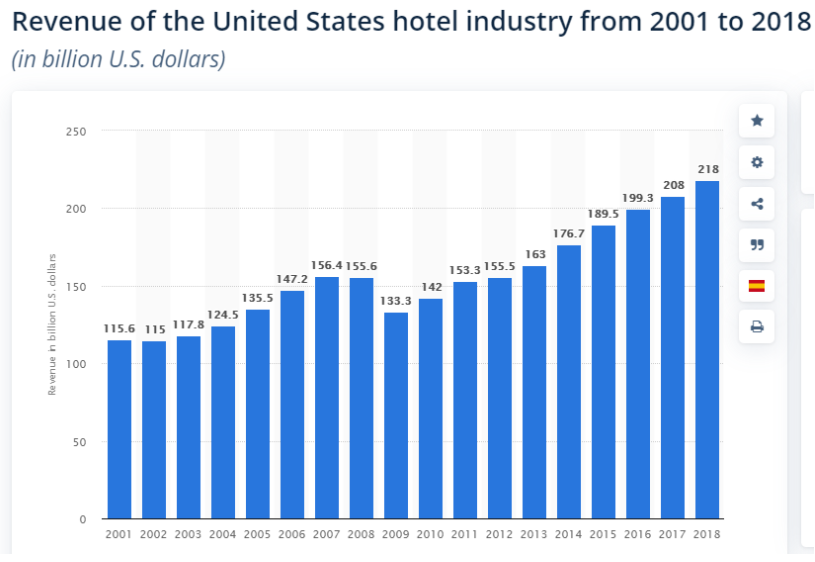
\includegraphics[scale=0.4]{hotelstats.png}
    \caption{Hotel revenue data from statistisa, source \href{https://www.statista.com/statistics/245841/total-revenue-of-the-us-hotel-industry/}{here}}
\end{figure}
\paragraph{}
We view the pandemic not as a permanent detriment, but merely as a temporary recession. We base our prediction on the figure which shows during the 2008 recession, which shows despite a drop, in 2008, the market corrected itself in just 5 years, bouncing back fully and going on to maintain consistent growth. We hope to use this correctional period as an opportunity to build a powerful tool to assist consumers in booking and finding hotels when the industry inevitably bounces back, and see this as our own opportunity to disrupt the booking industry with a powerful piece of online software. 

\subsection{Goals}
\paragraph{}
Our project has three primary service goals which help quantify how well our services meet the needs of our users:
\begin{enumerate}
    \item Easy and fast way to search hotels based off of parameters like date and location. This service goal posits that the search page must load in under 3 seconds and a search must take no longer than 5 seconds. 
    \item Ability for users to quickly book hotels. If a user knows what they want, the average time between a search and a book should be around 10 seconds. This ensures our service is straightforward and does what it's supposed to do without offering distractions.
    \item Ability for users to create accounts and favorite hotels. We will consider this feature successful if we get 1 account creation per 20 bookings. 
\end{enumerate}

\section{Stakeholders \\(Written by Nicholas Tymeson)}
\subsection{Our Users}
\paragraph{}
Users have a variety of needs and personal requirements when searching for hotels. The duration of their stay, like-minded customer reviews, number of people travelling, accommodating features and location, all play a crucial role in the hotel booking process. Some users may be very particular about what they’re looking for, while others may only be concerned about proximity to their destination’s attraction. Users might highly value the cleanliness of the hotel, which is a detail that would strongly influence many decisions to book or look elsewhere. Some may value accommodating features such as a fitness center, complimentary meals or service quality. Every user has a personal preference and this why hotel booking is always a process.
\subsection{User Characteristics}
\paragraph{}
Some characteristics in particular might include health/fitness oriented users, users focused on cleanliness, friendly and outgoing - might want to interact with staff, people who cook frequently, people focused on safety, and those with physical disabilities. With all of these characteristics taken into account, hotels must have a variety of accommodations such as fitness centers, handicap accessible rooms and facilities, friendly and approachable staff, mini kitchens and clean rooms.

\section{Mandated Constraints\\ (Written by Ed Tomlinson)}
\subsection{Solution Constraints}

\subsubsection{Browser Portability}
\textbf{Description:} Garlic Hotel Search shall operate on all major internet browsers.\newline
\textbf{Rationale:} The users will use specific browsers and should not have to download a new one to operate Garlic Hotel Search.\newline
\textbf{Fit Criterion:} Garlic Hotel Search will be tested on Mozilla Firefox, Google Chrome, Safari, and Edge.

\subsubsection{Device Portability}
\textbf{Description:} Garlic Hotel Search shall operate on any screen size.\newline
\textbf{Rationale:} Users will use a specific device to view the product and should be able to view all key components.\newline
\textbf{Fit Criterion:} Garlic Hotel Search will be run on an emulator of all major screen sizes.

\subsubsection{Relevant Results}
\textbf{Description:} Garlic Hotel Search will show only relevant results from the search.\newline
\textbf{Rationale:} Users searched for specific parameters and should not see results not relevant to that search.\newline
\textbf{Fit Criterion:} All search results will match parameters given during search.

\subsubsection{Account Security}
\textbf{Description:} Garlic Hotel Search will only let clients with username and password log into a specific account.\newline
\textbf{Rationale:} User Accounts belong to a specific user and should not be accessed by others.\newline
\textbf{Fit Criterion:} The password for the account shall be unique and hashed.

\subsubsection{Personalized Results}
\textbf{Description:} Garlic Hotel Search search results will include relevant user favorited hotels.\newline
\textbf{Rationale:} A user can favorite a hotel, and that hotel should appear in future searches when relevant.\newline
\textbf{Fit Criterion:} Favorite hotels should appear in results from searches in or near their city.

\subsection{Implementation Environment}
\paragraph{}
Garlic Hotel Search shall run an internet based server. When the site is launched it will run on an internet based server so Users can access at any time. Garlic Hotel Search’s database will run on a MySQL server. The database may need to be accessed at any time. Without buying hardware to create our own database servers, a cloud based server will be the best option.

\subsection{Partner or Collaborative applications}
\paragraph{}
Garlic Hotel Search will use web data scraped from Expedia. Garlic Hotel Search does not meet the requirements necessary to use a hotel search API. Therefore we will have to scrape data from an existing site. This data will be used to complete our search requests.

\subsection{Off the shelf Software}
\paragraph{}
This is a list of OTS software used (eg bootstrap):
\begin{itemize}
    \item Garlic Hotel Search is built using \textbf{Node.js}. Node.js lets code be run concurrently and will allow multiple users to use the website simultaneously.
    \item \textbf{Express.js} is used to create Garlic Hotel Search site routing. Express.js also provides APIs and middleware used to create calls from our database and backend.
    \item  \textbf{MySQL} is used for Garlic Hotel Search’s database. MySQL is used to store our database on cloud. It can be used in the future to create powerful queries data if we create our own database of hotels and their corresponding information.
    \item \textbf{BCrypt} is used to encrypt and store user passwords in Garlic Hotel Search’s database.
    \item \textbf{Concurrently} is used to run multiple database queries simultaneously.
\end{itemize}

\subsection{Schedule}
\paragraph{}
This is a list of the remaining sprints that need to be accomplished and when:

\begin{enumerate}
    \item Sprint 2 Objectives must be completed by 10/20. Sprint 2 will ensure Garlic Hotel Search is on track. Missing objectives can be pushed to Sprint 3 but will delay the project. Too many missing objectives will affect our grade, and could affect the quality of the finished website. 
    \item Sprint 3 Objectives must be completed by 11/10. Sprint 3 is the final sprint before completion. Most objectives for Garlic Hotel Search should be completed by this deadline. Remaining time in term should be used for testing and finishing touches to the website. Any missing objectives must be completed ASAP otherwise we risk submitting an incomplete project.
    \item Garlic Hotel Search is due on 11/19. Final product must be submitted by this date. All objectives must be completed or they will not be part of the final version of Garlic Hotel Search. An incomplete project will affect the grade and could potentially be cause for the group failing.
\end{enumerate}

\section{Naming Conventions and Terms\\ (Written by James Oswald)}
\paragraph{}
Our project's vocabulary is mostly technical in nature, contains no acronyms and is entirely for the purpose of talking about implementation. The few non-technical terms we use are in relation to speeding up writing business requirements, and pieces of software used by our group.
\subsection{Non-technical / Tool Glossary}
\begin{itemize}
    \item \textbf{User:} Anyone using the application.
    \item \textbf{User Story ID:} A concise identifier for a user story.
    \item \textbf{Expedia:} The website we scrape hotel data from.
    \item \textbf{Overleaf/Latex:} Software used for formatting our internal documents. 
    \item \textbf{Discord:} Communications Platform for VOIP and Messaging we use for internal communication and SCRUM Meetings.
    
\end{itemize}
\subsection{Technical Glossary}
\subsubsection{Frontend Glossary}
\begin{itemize}
    \item \textbf{Client:} The user's device. 
    \item \textbf{Client Code:} Code that runs on the client. 
    \item \textbf{Client Side:} Environment that runs client code, a web browser. 
    \item \textbf{Fetch:} the JS Fetch API used frontend to communicate with the backend over HTTPS.
    \item \textbf{Client Router:} React.js Router. 
\end{itemize}
\subsubsection{Backend Glossary}
\begin{itemize}
    \item \textbf{Server:} The hosting device. 
    item \textbf{Server Code:} Code that runs on the server.
    item \textbf{Server Side:} Environment that runs server code, node.js and python3 in a shell. 
    \item \textbf{Server Router:} Express.js Routing.
    \item \textbf{Endpoint Call:} A faux page requested by the fetch API and processed by express from the front end when making a server request. 
    \item \textbf{Endpoint:} The actual method that runs server side when a request is made to preform an action from the client. 
    \item \textbf{Listing:} The object that stores a hotel listing on the backend and is fully passed to the frontend when a search is made.
\end{itemize}

\subsubsection{Project Glossary}
\begin{itemize}
    \item \textbf{Setup:} The process to rebuild the project after new commits are made, named after the "Setup.bat" script in the project root that updates node packages and rebuilds the react frontend.
    \item \textbf{Test DB:} The test database, setup on a separate server to test the application works with a real SQL database. 
    \item \textbf{Cred File:} A special JSON file in the .gitignore that contains the database credentials. 
    \item \textbf{Compound Debug:} VS code debugging both the frontend and backend simultaneously. 
    \item \textbf{React Deletion:} When react compiles away a feature we wanted it to keep in the optimized build. 
    \item \textbf{User Code:} (Not to be confused with client code) Any code that deals with User features, creation, settings, updating, etc. All contained in one file called "userCode.js".
\end{itemize}


\section{Relevant Facts and Assumptions\\ (Written by Nicholas Tymeson)}
\paragraph{Assumptions}
The following is a list of fair assumptions to make about users:
\begin{itemize}
    \item It is Fair to assume users are looking for hotels close to a particular location.
    \item It is Fair to assume users have a given price range based on the duration of their stay.
    \item It is Fair to assume users lean towards certain hotels with certain features, policies and reviews.
    \item It is Fair to assume users have a certain number of children and adults that will be staying.
\end{itemize}
  
\section{Scope \\(Written by Paing Htet)}
\begin{figure}[H]
    \centering
    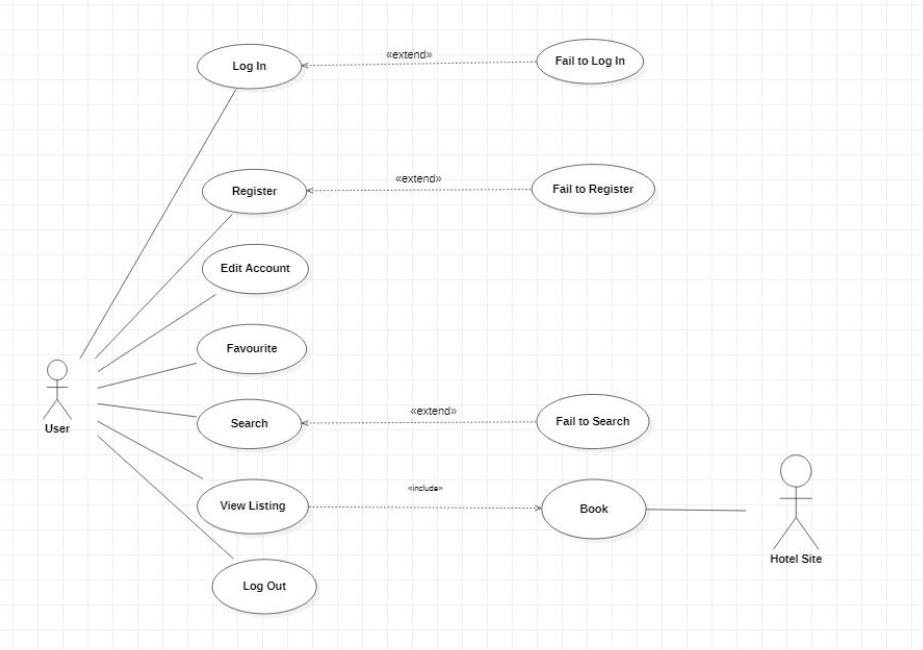
\includegraphics[scale=0.4]{usecase.png}
    \caption{Our Updated Use Case Diagram}
\end{figure}

\section{Functional Requirements \\ (Written by Kyler Randall)}
\subsection{Functional Requirements}
\subsubsection{Sprint 1}
\textbf{User Story ID}: Search Implementation\newline
\textbf{Description:} The product shall allow the user to enter an address and have the correct hotel listings displayed. Test API data needs to be displayed when the user enters an address and hits search. \newline
\textbf{Fit Criterion:}
\begin{enumerate}
    \item The user accesses the web page.
    \item The user is able to type in an address in the main search bar.
    \item The user is able to hit search and have test hotel data displayed un-styled below the search bar if there are matches. If no matched hotel is found a message is displayed saying “No results”
    \item The search is logged server side
\end{enumerate}

\subsubsection{Sprint 2}
\textbf{User Story ID}: Account Creation and Management\newline
\textbf{Description:} The User needs to be able to register for an account as well as update their account information.\newline
\textbf{Fit Criterion:}
\begin{enumerate}
    \item The user accesses the web page.
    \item The user accesses the register page.
    \item The user is able to create an account using their email.
    \item The user is prompted with a “Account Successfully Created” message.
    \item The user has access to an account management page when they are logged in.
    \item The user is able to update their account information and click save to have this info permanently updated in the database.
    \item When a user attempts to login the system authenticates the credentials
    \item If the credentials fail the authentification the system displays a “Invalid Username/Password” Message. The system then allows the user to enter their credentials again.
    \item After a successful login the system will give the user access to the account management page.
\end{enumerate}

\noindent
\textbf{User Story ID}: Search Constraints\newline
\textbf{Description:} The User needs to be able to search for hotel listings using an address, number of Adults/Children and how many rooms they need.\newline
\textbf{Fit Criterion:}
\begin{enumerate}
    \item The user accesses the web page.
    \item The user selects how many adults/children will be staying as well as how many rooms they need.
    \item The user hits the search button and the hotels are listed below the search. If the there is no data that matches the search criteria a message is displayed saying “No Results”.
\end{enumerate}

\noindent
\textbf{User Story ID}: User Logout\newline
\textbf{Description:} The User needs to be able to logout of their account.\newline
\textbf{Fit Criterion:}
\begin{enumerate}
    \item When a user is logged in the system will display a logout button for the user to press.
    \item The user clicks the logout button and the system displays a message “Successfully logged out”.
    \item The system sends the user back to the homepage.
    \item The system restricts the user’s access to the account management page and now no longer displays their favorites.
\end{enumerate}

\noindent
\textbf{User Story ID}: Price Listing \newline
\textbf{Description:} Hotel listings need to show pricing based on a selected currency and how many days the hotel will be booked for.\newline
\textbf{Fit Criterion:}
\begin{enumerate}
    \item The user accesses the web page.
    \item The user is able to select which currency they wish to have the pricing displayed as. As well as selecting how many days the hotel will be booked for. If the search criteria does not match a message is displayed “No Results”. 
    \item The system displays the hotel listings below the search and recalculates the pricing based on a currency conversion API.
\end{enumerate}

\subsection{Traceability Matrix}
\subsubsection{Sprint 1}
\noindent
\textbf{User Story:} I need to be able to see the homepage and navigate to other pages by typing their addresses into the search bar. This proves that basic routing and page creation with react has been implemented. \newline
\textbf{Notes:} The search bar is one of the main components of the site. This is a feature needed to be demoed for the first sprint. \newline
\textbf{Requirements:} PG. 1 - Provide a Search Bar \newline

\noindent
\textbf{User Story:} I need to be able to access the user database with SQL queries. This proves that the database is set up and ready to be integrated into the application backend. \newline
\textbf{Notes:} Basic functionality for a user to make an account. A later sprint will account for editing of user info. \newline
\textbf{Requirements:} PG. 1 - Create a Login/Register Page \newline

\noindent
\textbf{User Story:} I need to be able to make test API calls using functionality exposed to the backend. This proves that the API has been selected and is ready to be integrated into the backend \newline
\textbf{Notes:} Mock data has been made and displayed on the main page. \newline
\textbf{Requirements:} PG. 1/2 – Hotel Listings Should \newline

\subsubsection{Sprint 2}

\noindent
\textbf{User Story:} I need to be able to register for an account as well as update my account information. This information includes the account profile picture, password, and username/email \newline
\textbf{Notes:} Add onto the account creation feature made during sprint 1. \newline
\textbf{Requirements:} PG. 2 - An account Editing page if the user is logged in
\begin{itemize}
    \item A way to change passwords
    \item Change Name/Email
    \item Change Photo
    \item Have changes be confirmed with a save button and redirect to the main page afterwards.
\end{itemize}

\noindent
\textbf{User Story:} I need to be able to search for hotel listings based on address. I also need the option to search based on how many adults/children and how many rooms. \newline
\textbf{Notes:} Sprint 2 to will build upon the search bar functionality created is Sprint 1. \newline
\textbf{Requirements:} PG. 1 – Provide a Search Bar
\begin{itemize}
    \item The search bar will take a Country and City parameters
    \item There should also be dropdown menus for how many adults and kids will be attending the hotel, as well as how many rooms.
\end{itemize}

\noindent
\textbf{User Story:} I need to be able to show pricing for hotels based on a selected currency and how many days the hotel will be booked for. \newline
\textbf{Notes:} Sprint 2 will build upon the search bar functionality as well as building upon ways in which the hotel listings can be displayed. \newline
\textbf{Requirements:} PG. 1 – Provide a Search Bar and PG. 1/2 - Hotel Listings Should
\begin{itemize}
    \item Have a dropdown menu for the user to select a currency (Default should be USD)
    \item On the side of the Search Bar include some boxes where the user will be able to plug in the dates when the user will move in and move out.
\end{itemize}

\noindent
\textbf{User Story:} Frontend data display works and displays data. \newline
\textbf{Notes:} For the most part the hotel listing info will remain unstyled until Sprint 3. Sprint 2 will focus on getting the “Required” attributes displayed. \newline
\textbf{Requirements:}\newline PG. 1/2 – Hotel Listings Should:
\begin{itemize}
    \item Be preferably rendered in the same page (Desired).
    \item Be Listed by Ratings by default and must have option to change the sorting filter (Required).
\end{itemize}
\noindent
Each Listing much have:
\begin{itemize}
    \item Name of the Hotel, and Room/Bed Size Info (Required).
    \item Rating System from 1-5 or 1-10 (Required).
    \item A Pre-Tax Price per Night (Required).
    \item A Pre-Tax Overall Price (Desired).
    \item Post-Tax Prices (Optional if the user provides their current location on their browser).
    \item The Hotel’s address, as well as a google maps link (Required).
    \item A Box that includes a list of pictures of each room (Required).
    \item A button that will redirect them either to a booking site online or that hotel’s website where the user can book the room or prompt the user to pay on the website itself (Website will be hosted outside of University Domains, so this is okay with University Policy). (Required) (Specific choice is up to the Team).
    \item A check in and check out time (Required).
    \item Hotel Phone Number (Desired)
    \item All Services provided by the hotel (Desired)
    \item Any Policies necessary to be shown (ex. “Pets not allowed”) (Desired)
    \item Any activity centers in the hotel (ex. Library, Gym etc) (Desired) General features of the hotel. (Required)
\end{itemize}

\subsubsection{Sprint 3}

\noindent
\textbf{User Story:} I need to be able to save hotel listings to my favorites. \newline
\textbf{Notes:} Users can only favorite hotels if they are registered. \newline
\textbf{Requirements:} PG. 1 – Create a Login/Register Page
\begin{itemize}
    \item Using an account will grant privileges to save certain hotel listings on the account.
\end{itemize}

\noindent
\textbf{User Story:} I need to have the hotels displayed in a an organized and visually appealing way. \newline
\textbf{Notes:} Most data will already be displayed. Sprint 3 will focus on styling the hotel listing information. \newline
\textbf{Requirements:} PG. 1/2 – Hotel Listings Should:
\begin{itemize}
    \item Choose the most important of these characteristics to render alongside other listings, and when clicking an individual listing’s name, generate the detailed version of that hotel and room. The ideas above are simply a guideline for all the info Required and/or Desired.
\end{itemize}

\noindent
\textbf{User Story:} I need to be able to be brought to a site where I can book a hotel \newline
\textbf{Requirements:} PG. 1/2 – Hotel Listings Should:
\begin{itemize}
    \item A button that will redirect them either to a booking site online or that hotel’s website where the user can book the room or prompt the user to pay on the website itself (Website will be hosted outside of University Domains, so this is okay with University Policy). (Required) (Specific choice is up to the Team)
\end{itemize}

\section{Non-functional requirements \\ (Written by Ethan Seligman)}
\subsection{Appearance}
\paragraph{}
Appearance should have a modern and responsive design that will engage any user with a “wow” factor. Color palette should include as many neutral (or close to neutral) colors with a distinctive non-neutral color as the primary color. Buttons, links, and other similar components will have the primary color (in our case green) to attract the user's eyes.
\subsection{Usability}
\paragraph{}
Consumers will be able to search for hotels to book without any ad clutter, tracking data, and similarly annoying features that most hotel websites have.Page layout will be straightforward and easy to navigate for users of all ages.
\subsection{Performance}
\begin{itemize}
    \item Unnecessary API and database queries will be avoided ensuring optimal performance. 
    \item Minifying Javascript, CSS, and HTML will be done to optimize page loading times.
    \item Only compressed images will be used. Images > 1MB will not be used.
\end{itemize}

\subsection{Security}
\begin{itemize}
    \item All sensitive user data will be hashed and salted using the bcrypt algorithm.  
    \item Spam prevention will be done to ensure users do not flood our back-end with requests. 
    \item Sanitization of user inputs will also be done to ensure no SQL injections will occur. We are accomplishing this by using prepared statements to query our SQL database.
    \item Only users with privileged web server access will be able to see the database tables and their rows.
\end{itemize}

\section{Formatting Notes \\ (Written by James Oswald)}
\paragraph{}
This document was formatted using Latex and the .tex source code can be found on the UA Team Garlic Github in the \href{https://github.com/UAlbany-Team-Garlic/GHS-SRS-Document}{GHS-SRS-Document Repository}. The original unformatted document can also be found there.

\end{document}
